\documentclass[a4paper,11pt]{article}


\usepackage{color}
\usepackage{array}
\usepackage{amsmath,amssymb}
\usepackage{graphics}
\usepackage[utf8]{inputenc}
\usepackage[spanish]{babel}


\addtolength{\textwidth}{2cm}
\addtolength{\hoffset}{-1cm}


\title{QSudoku}
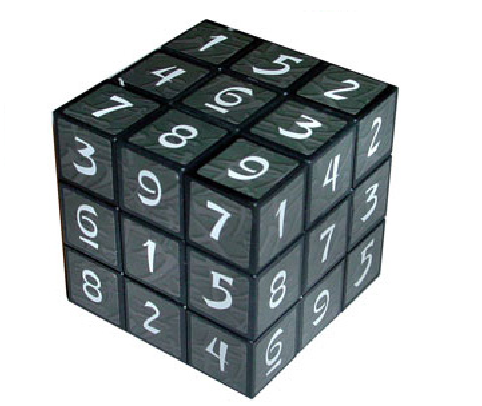
\includegraphics{sudo.png}


\title{Qsudoku}
\author{Ramón Carrillo, Juan Mite, Esteban Muñoz}

\begin{document}
\maketitle
\tableofcontents

\section{Introducción}
Es una aplicación realizada en lenguaje c++, utilizando el IDE Qt Creator, es una adaptación de famoso Sudoku, un pasatiempo que se publicó por primera vez a finales de la década de 1970 y se popularizó en Japón en 1986, dándose a conocer en el ámbito internacional en 2005 cuando numerosos periódicos empezaron a publicarlo en su sección de pasatiempos.

\subsection{Descripción}

El objetivo del sudoku es rellenar una cuadrícula de 9 x 9 celdas (81 casillas) dividida en subcuadrículas de 3 x 3 (también llamadas "cajas" o "regiones") con las cifras del 1 al 9 partiendo de algunos números ya dispuestos en algunas de las celdas. Aunque se podrían usar colores, letras, figuras, se conviene en usar números para mayor claridad, lo que importa, es que sean nueve elementos diferenciados, que no se deben repetir en una misma fila, columna o subcuadrícula. Un sudoku está bien planteado si la solución es única. La solución de un sudoku siempre es un cuadrado latino, aunque el recíproco en general no es cierto ya que el sudoku establece la restricción añadida de que no se puede repetir un mismo número en una región. 

\section{Desiciones de Diseño}
	Una de las cosas que destaca a nuestro proyecto es la interfaz de usuario desde ahí se puede notar de una forma rápida las decisiones de diseño que hemos considerado para la implementación de algoritmos, ventanas, efectos, etcétera.

	“Simpleza” sobre “Mucho de todo”, es lo que caracteriza a QSudoku, simpleza e intuitivo, es decir el usuario promedio no necesitará leer el manual para saber lo que tiene que hacer en el juego, solo hace falta un poco de sentido común, aun así sabemos que le sentido común no es el más común de los sentidos por ende hemos implementado un sistema de etiquetas interactivas en los botones (tooltips).

	Como dijimos antes la simpleza prevalece en QSudoku, hay que aclarar también que simpleza no quiere decir cosas a medias, sino más bien indicador de buen estilo y principio de desarrollo y hacemos referencia a la frase de Guillermo de Ockham: “lo más simple es lo mejor”.

\section{Algoritmos}
	Para la realización de QSudoku hemos implementados una serie de algoritmos que cumplen funciones específicas, los cuales fueron hechos de tal manera que fueran simples pero efectivos al momento de cumplir con el propósito al cual fueron destinados, dichas funcionalidades son descritas a continuación:

\subsection{Algoritmo de generación del tablero}
\subsubsection{Descripción}
Algoritmo de generación del tablero de Qsudoku o “Sudoku engine” como esta descrito en el repositorio Git-hub del proyecto, es precisamente eso, es el motor del juego, este genera un tablero a partir de un tablero antes resuelto o tablero base.

\subsubsection{¿Por qué lo escogimos?}
Lo cierto es que es muy complicado que una máquina genere tableros de sudokus porque para esto debe de tener una serie de consideraciones, estas consideraciones se toman para no generar tableros con varias soluciones, es decir, un tablero de sudoku está bien hecho sí y solo sí tiene una sola solución, además nunca se debe dejar que una columna o una fila este llena en su totalidad.
	Debido a las consideraciones antes expuestas y a las decisiones de diseño tomadas con respecto a simpleza, hemos implementado el siguiente algoritmo:

\subsubsection{Explicación}

1.	Tomamos un tablero lleno, resuelto anteriormente.


\centerline{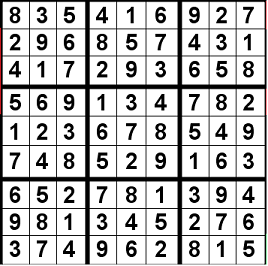
\includegraphics{tab.png}}
\centerline{figura 3.1: Tablero vacío.}\\
2.	Generamos los aleatorios los cuales nos servirán para intercambiar, filas, columnas, cuadriculas verticales u horizontales que son la agrupación ordenada y consecutiva de 3x9 celdas, celdas que son la unidad mínima posible en el tablero y es donde van ubicado los números.

\centerline{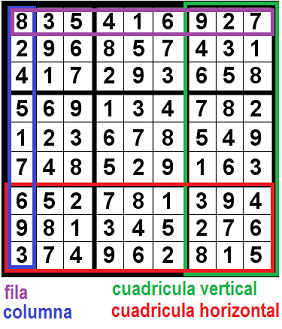
\includegraphics{sudoResuelto.png}}
\centerline{figura 3.2: Definiciones.}

3.	Establecemos las reglas para entreverar el tablero.\\
-Solo se podrán mover columnas que pertenezcan a la misma cuadricula vertical.\\
-Solo se podrán mover filas que pertenezcan a la misma cuadricula horizontal.\\
-Solo se podrán mover cuadriculas verticales así como se muestra en el ejemplo, nunca se podrá intercambiar una cuadricula vertical con una horizontal.\\
-Si se decide cambiar una columna vertical por una horizontal o viceversa se tendrá que hacer lo mismo para todas.\\
4.	Hacemos los intercambios permitidos.\\

\centerline{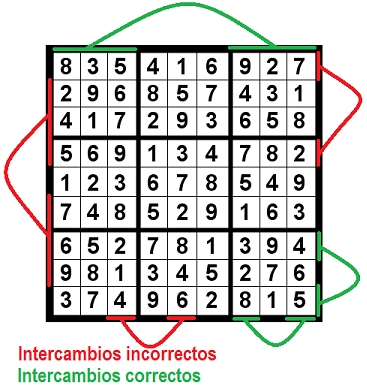
\includegraphics{sudoRe.png}}
\centerline{figura 3.3: Intercambios}

5.	Fin del algoritmo

\subsection{Algoritmo de dificultad del tablero}
\subsubsection{Descripción}
	Una vez lleno el tablero con el algoritmo descrito anteriormente, se procede a dejar los espacios que el jugador deberá llenar, esto lo hará aleatoriamente también y para que le tablero no se queden huecos ni tampoco queden columnas ni filas totalmente llenas, hemos decidido implementa el siguiente algoritmo:
\subsubsection{Explicación}
En los diferentes niveles de dificultad Fácil, intermedio, difícil, se dejará 36, 45, 63 espacios en respectivamente, también si una fila o columna tiene menos de 3 valores en sus celdas ya no se le podrá sacar más valores.
\subsubsection{¿Por qué lo escogimos?}
	Escogimos esta manera de darle dificultad al tablero luego de ponerlo a prueba, esto porque al inicio no estábamos convencidos de que era efectivo, es decir, es tan simple que en la teoría da lugar a dudas, pero una vez puesto en práctica resulto ser efectivo, limpio y cubrió nuestras expectativas.

\subsection{Algoritmo de validación de tablero}
\subsubsection{Descripción}
Una vez que el jugador llene todo el tablero podrá presionar el botón de verificación o final de juego, este correrá la una validación descrita por el algoritmo que se describe a continuación:

\subsubsection{Explicación}
1.	Se recorre cada columna del tablero, se suman y se multiplican sus valores, el resultado debe de dar 45 y 362880 respectivamente.
2.	Se recorre cada fila del tablero, se suman y se multiplican sus valores, el resultado debe de dar 45 y 362880 respectivamente.
3.	Se recorre cada cuadra de 3x3 del tablero, se suman y se multiplican sus valores, el resultado debe de dar 45 y 362880 respectivamente.
4.	Se verifica cada uno de estas sumas y multiplicaciones, si la suma o la multiplicación de cada una de estas no da el número entonces lanzará un cuadro de dialogo con el mensaje: Tablero no valido, caso contrario se mostrará tablero valido.

\subsubsection{¿Por qué lo escogimos?}
Aparte de ser muy sencillo de implementar es preciso, aunque pensamos que no es tan óptimo debido a todos los recorridos que tiene que hacer, pero en la práctica perfectamente, no hay retrasos significativos, no se cuelga y funciona perfectamente es efectivo y confiable.

\subsection{Algoritmo de puntuación}
\subsubsection{Descripción}
	Para que el Jugador registre su puntuación deberá terminar un juego, es decir, deberá llenar un tablero y que éste esté lleno correctamente, para darle al jugador su respectivo puntaje consideramos los siguientes criterios
1.	La dificultad escogida
2.	El tiempo que le tomo resolverlo

\subsubsection{Explicación}
	Una vez presionado el botón de verificación se corre el algoritmo de validación, si éste devuelve una respuesta positiva se le asignará al jugador su respectivo puntaje, el mismo que dependerá del tiempo y de la dificultad escogida, si el tablero no es válido entonces se regresará a la partida. La puntuación final es igual a la multiplicación de su tiempo y el factor dificultad, para fácil es 1, para intermedio es 0.75 y para difícil es 0.5. 
\subsubsection{¿Por qué lo escogimos?}
Seleccionamos esta manera de asignar puntaciones puesto que es la más lógica y realmente es lo más destacable de un jugador, de tal manera que, si un jugador no llena el tablero, no podrá ser calificado, por otro lado si lo llena en poco tiempo y en modo difícil tendrá una puntuación más alta.

\subsection{Algoritmo de encriptación}
\subsubsection{Descripción}
Para salvaguardar la integridad de los datos, el juego guarda las partidas y los puntajes encriptados, para esto usamos un la operación XOR aprovechando sus propiedades matemáticas.


\centerline{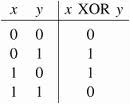
\includegraphics{xor.png}}
\centerline{figura 3.4: tabla de verdad de XOR }

\subsubsection{Explicación}
1.	Se genera una “clave” al azar esta clave es un conjunto de unos y ceros
2.	Se lleva de caracteres a unos y ceros el contenido que se va a guardar
3.	Se hace la operación XOR ente la clave y los caracteres ya en binario, la clave se ira repitiendo secuencialmente para cubrir toda la información a guardar
4.	Se guarda en un archivo externo.
5.	Fin.

\subsubsection{¿Por qué lo escogimos?}
	Escogimos este método, porque es seguro, la única posible falla es que si se sabe cómo se  guardan los datos, es decir, el orden en que se guardan, si se conoce la “clave”, la cual se genera aleatoriamente al momento de guardar, entonces solo así se podrá acceder a los datos.


\section{Manual de usuario} 


\subsection{Pasos de la aplicación}
Al lanzar la aplicación se mostrará una pantalla de inicio la cual permitirá al jugador registrarse, escoger la dificultad de juego, ver las estadísticas de juegos pasados, desarrolladores e iniciar su juego con los requisitos que especificó al inicio.


\centerline{\subsection{Pantalla inicial}}
\centerline{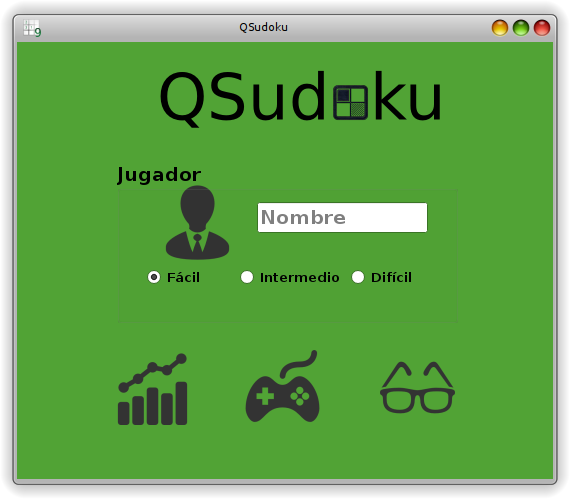
\includegraphics{ini.png}}
\centerline{figura 4.1: Ventana principal}
Ventana que se lanza al iniciar el juego.
\subsection{Preferencias}

\centerline{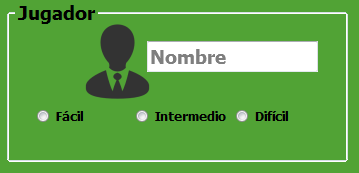
\includegraphics{nombre.png}
\centerline{figura 4.2: niveles de dificultad}

Aquí el jugador dejará su nombre y escogerá la dificultad con la que quiera fijar el tablero, si el jugador no fija una dificultad, el juego le asigna una facil por default.
\subsection{Juego nuevo}

\centerline{
\includegraphics{nuevoICO.png}
\centerline{figura 4.3: Botón Jugar}
Al presionar aquí el jugador empezará con el juego.
\subsection{Estadísticas}

\centerline{
\includegraphics{estadistICO.png}}
\centerline{figura 4.4:Botón  Estadídticas}


Al presionar aquí el jugador verá las estadisticas.

\subsection{Desarrolladores}

\centerline{
\includegraphics{develoICO.png}}
\centerline{figura 4.5: Botón desarrolladores}

Al presionar aquí el jugador verá información de los desarrolladores.

\subsection{Botón Home}

\centerline{
\includegraphics{home.png}}
\centerline{figura 5.5: Botón Home }

Al presionar aquí el jugador regresará a la pantalla de inicio.

\section{Ventanas}


\subsection{Juego Nuevo}

\centerline{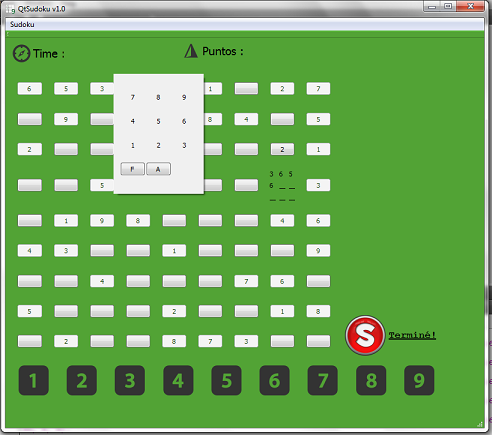
\includegraphics{tablero.png}}
\centerline{figura 5.1: Tablero sudoku}
\subsection{Barra de menú}

\centerline{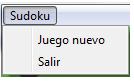
\includegraphics{barra.png}}
\centerline{figura 5.2: barra de menú}

En este menú el jugador contará con dos opciones, la funcionalidad de las mismas se detalla a continuación.
\subsection{Sudoku /Juego Nuevo}
El jugador podrá llenar un nuevo tablero, es decir reiniciar la parida desde Cero.
\subsection{Sudoku /Salir}
El jugador podrá salir del juego dando clic aquí, lo hará sin guardar partida simplemente cancelará su juego.
\subsection{figura 5.3: Botón Terminé!}

\centerline{
\includegraphics{termine.png}}
\centerline{figura 5.4: Boton verificar tablero}

Al presionar aquí el jugador comprobará si llenó su tablero correctamente o no.
\subsection{Desarrolladores}

\centerline{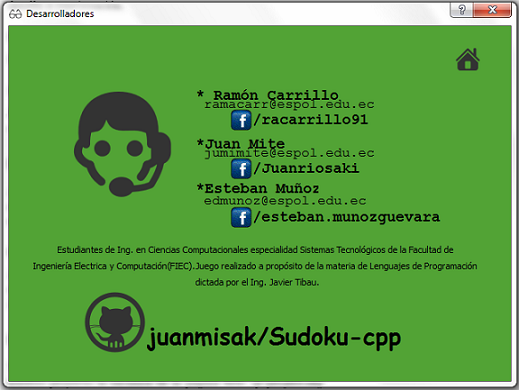
\includegraphics{pagdesa.png}}
\centerline{figura 5.5: Ventana Desarrolladores}

Aquí se muestra información acerca del juego como por ejemplo la versión del juego, desarrolladores, ubicación del repositorio Git Hub y la dirección de facebook de cada uno de ellos.
Juan Mite, Daniel Muñoz, Ramón Carrillo, Estudiantes de la Escuela Superior Politécnica del Litoral a propósito de la materia de Lenguajes de programación dictada por el Ing. Javier Tibau profesor de la Facultad de Ingeniería Eléctrica y Computación.  
\subsection{Estadísticas}

\centerline{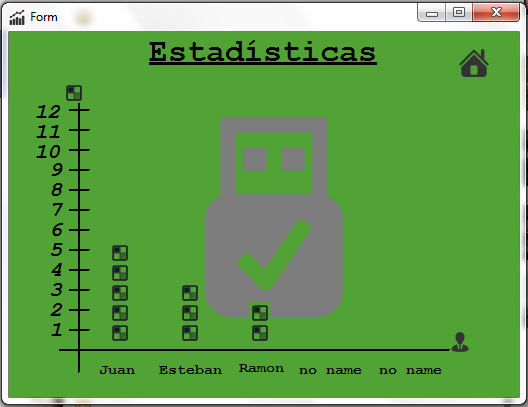
\includegraphics{estadist.png}}
\centerline{figura 5.6: Ventana Estadística}

En esta ventana el jugador verá las puntuaciones de los 5 jugadores que han obtenido las mejores puntuaciones, en la esquina superior derecha hay un botón que lo reresará al Home.



\section{Bibliografía}
Toda la ayuda e información sobre de las herramientas que necesitamos para desarrollar nuestro proyecto la sacamos de la pagina web:
qt-project.org
\section{Referencias}\\
www.fceia.unr.edu.ar/lcc/cdrom/Instalaciones/LaTex/latex.html \\
www.kabytes.com/diseno/decisiones-de-diseno-web/ \\
es.wikipedia.org/wiki/Navaja_de_Ockham/ \\
es.wikipedia.org/wiki/Cifrado_XOR/ \\

\end{document}

